\documentclass{svproc}
\usepackage{url}
\usepackage{cite}
\usepackage[ruled]{algorithm2e}
\usepackage{graphicx}
\usepackage{amsmath}
\usepackage{amssymb}
\usepackage{algpseudocode}
\usepackage{todonotes}
\usepackage{subfig}

\def\UrlFont{\rmfamily}


\begin{document}
    \mainmatter
    \title{CS7IS2 - Analysis of Artificial Intelligence Algorithms On The Game 2048
    }
    \author{Rohan Anand, Rohan Bagwe, Sameer Karode, Kavithvajen Kamaraj}

    \institute{Trinity College Dublin \newline
        \email{anandr@tcd.ie}, \email{bagwer@tcd.ie}, \email{karodes@tcd.ie}, \email{kamarajk@tcd.ie}}

    \maketitle

    \begin{abstract}
        Video games and puzzle problems are widely used in the field of Artificial Intelligence(AI) to see if machines are truly intelligent enough to understand what it takes to win a game. This paper uses the game 2048 to analyse how some popular reinforcement learning algorithms perform. The AI agents are guided using Monte-Carlo Tree Search, Expectimax, Greedy First and Q-Learning and their results are compared with how the agent would perform against Random algoritm as baseline. The results of the experiments show that Expectimax is the best algorithm out of these to win a game of 2048. It is also noted that algorithms with a greedy approach perform better than the ones that play a random move like Monte-Carlo Tree Search.
        
        \keywords{Artificial Intelligence, 2048 Game, Deep Q Network, Monte Carlo Tree Search, Expectimax Search}
    \end{abstract}

    \section{Introduction}

Games have always been used to demonstrate the prowess of Artificial Intelligence algorithms, a few good examples are IBM’s Deep Blue which was trained to play Chess \cite{deepBlue}, and AlphaGo which was trained to play the board game Go \cite{alphago}. Besides these popular examples, AI agents have been successful in playing complex video-games such as Starcraft \cite{starcraft}. It is useful to test AI algorithms on games as games provide a set of rules and rewards that makes it easy to set a goal for the agent. This works towards maximising the possibility of achieving the highest reward value. Due to the constraint laid by the game, it becomes easy for humans to track the development of the AI agent. Every game is modeled as a search problem with a heuristic evaluation function. This enables an AI agent to find the optimum solution for solving the game, making games the perfect test-bed for Artificial Intelligence algorithms.

% The game was released to the public in 2014 as free and open-source software, and it quickly became the most popular game in the market when mobile versions of the game were released \cite{wiki_2048}

The game chosen in this paper is 2048 \cite{2048}. It is a non-deterministic, single-player game that was developed by Gabriele Cirulli. The game is interesting due to its simple controls and yet hard to master. The game requires the player to have some sort of intelligence and an ability to look ahead of moves to determine what would lead them to go on and win the game, thus making it a perfect problem for an AI agent to solve. Also, 2048 can be clearly shown as a Markov Decision Process which provides an ideal platform to compare and contrast different AI reinforcement learning techniques \cite{jaskowski, pedagogy}.

Four algorithms have been chosen to be implemented and analysed in this paper - Greedy First Algorithm, Monte-Carlo Tree Search, Expectimax Search and Q-Learning. The performance of each of these algorithms is measured and compared against each other. The goal for the AI agent is to find the optimum solution to win a game of 2048 and achieve the best possible score.

    \section{Related Work}

    Expectimax is a recursive depth-limited tree search algorithm that does not treat the game as adversarial \cite{Maryam}. Adversarial search is performed in an multi-agent environment where two agents play against each other and try to explore and evaluate the shared search space for the solution ahead of each other. An agent decides the move to be played by playing all response moves of the opponent concerning every possible move of the agent. The most common example is the Mini-Max algorithm \cite{7162574, Dan} that uses an adversarial search to evaluate each move in terms of loss and gain for one of the agents. Each agent evaluates the search space such that the opponent agent gets the minimum benefit thereby increasing their reward. Adversarial Search is widely used in the Zero-sum games (Ex. Tic-Tac-Toe) where complete information about the game’s state is available. 
    
    However, this approach is not suitable for creating an AI agent to play the 2048 game as the knowledge of the game is not perfect. Since the tiles spawned are at random they are not necessarily targeted to the worst empty cell on the board. In Expectimax search, at every state of the game board, the maximum expected utility \cite{Maryam} chooses the next move to be played with a maximum fitness calculated through averaged depth limit search weighted by the probability of occurrence of that state (p=0.9 for 2-tile and p=0.1 for 4-tile) and a heuristic function. The chance nodes are administered by probabilities instead of choosing the maximum and minimum nodes in the case of the Mini-Max algorithm \cite{7162574}.
   
    Q learning and Deep Q-Networks (DQN) have been made more popular by \cite{mnih2013playing, mnih2015human}. In \cite{mnih2013playing}, the authors developed a DQN Agent to play 7 Atari games. They created a convolution neural network that takes the raw RGB input displayed by the game and attempts to output the move with the best possible reward. The model was able to beat all other algorithms in almost every game, even beating out human players. In \cite{szubert2014temporal}, the authors implement tuple networks as an AI agent to solve the 2048 game. This model was also used successfully in the games Othello \cite{jaskowski2014systematic} and Connect-4 \cite{thill2012reinforcement}. This approach uses Temporal Difference Learning (TDL) \cite{sutton1988learning}. Their approach was able to achieve the score 2048 in 98\% of games.
   
    \section{Problem Definition and Algorithm} \label{Game Explanation}

    2048 is played on a 4x4 grid where numbered tiles are present. The game randomly generated tiles with the numbers 2 and 4 after every move the player makes. The goal is to sum up same tiles with one another until 2048 is reached in at least one tile. The tiles are added by moving them either up, down, left or right. When a move is performed all the tiles in the grid move in the specified direction. The score starts at zero and is updated based on the value of the new tiles that are formed due to the combination of previous tiles (i.e., if two tiles with the value of 128 are combined, then the resulting tile will have the value of 256 and thus the score will also increment by 256 points). A player wins when they obtain a tile with the value 2048, but the game can continue to reach higher scores. The player is considered to have lost when all the tiles in the grid have a value and a move cannot be made to combine any of them.

    % \subsection{Random Moves Algorithm}

    % This paper started off with implementing an agent which randomly makes a move on game board out of 4 choices. It plays until the game is over. This is done several times while keeping track of the end game score. As this implementation is completely based upon random actions, the score serves as a baseline for evaluating rest of the other algorithms implemented in this project.
    
    % I dont think so???
    % Further, incremental improvements have been made so that agent can make informed decisions which will lead to a good score at the end of the run. 

    \subsection{Greedy First Algorithm}
    In this approach, an agent makes a move which is likely to generate a higher game score against a particular action. For instance, if the agent has 4 choices, it calculates the new game score for all the viable choices and then chooses an action which corresponds to the highest score. In cases where the moves generate the same score, the agent will randomly choose an action out of given choices.
    
    % \begin{algorithm}[t]
    %     \SetAlgoLined
    %     initialize\_gamegrid()\;
    %     \While{game\_over != True}{
    %         random\_move = get\_random\_move()\;
    %         gamegrid.play(random\_move);
    %     }
    %     \caption{Random Moves Algorithm}
    % \end{algorithm}
    
    
    Several heuristics are used to direct the optimization algorithm towards favourable positions. The various heuristics are weighted and combined into a positional score, which determines how ``good'' a given board position is. The choice of heuristics are as follows:
    
    \subsubsection{Heuristics} \label{heuristics}

    \begin{itemize}
        \item \textbf{{Max Score generated by immediate move:}}
        The agent can find the best move from a given set of actions based on the maximum score achieved. 
        %The calculation of score for the 2048 game is described in Section \ref{Game Explanation}.
        % Mathematically, equation for finding best move can be stated as follows.
        % \begin{equation} \label{max_score_equation}
        %              best\_move = argmax(score\_list\_of\_each\_move)
        % \end{equation}


        \item {\textbf{Number of Empty cells on game board after performing a move:}}

        %It takes into account the number of free tiles left. 
        If there are few empty tiles, then it’s likely that the game will end with low premature score. There is a penalty for having too few empty tiles, since options can quickly run out when the game board gets too cramped. This makes the agent choose the move that allows more free spaces by looking ahead. 

        \item {\textbf{Weight Matrix Multiplication Score:}}
        It has been observed that the agent can score well if the tiles with large values are maintained in the corner of the game grid. By using a weight matrix, we can mimic this strategy by setting the values of \textbf{W} such that the weight decreases from the top left to the bottom right. The equation \ref{weighted_score_equation} demonstrates that the agent will tend to make moves such that the bigger tiles are always closer to the corner than the smaller tiles, which agrees with the desired strategy.

        \begin{equation}
            \textbf{W} =
            \begin{pmatrix}
                7 & 6 & 5 & 4 \\
                6 & 5 & 4 & 3\\
                5 & 4 & 3 & 2 \\
                4 & 3 & 2 & 1 \\
            \end{pmatrix}
        \end{equation}

        \begin{equation} \label{weighted_score_equation}
        \textbf{ Weight\_Matrix\_score} = \textbf{W} \times \textbf{game\_grid\_matrix}
        \end{equation}

    

        % \item {\textbf{Monotonicity property}}
        % This heuristic tries to ensure that the values of the tiles are all either increasing or decreasing along both the left/right and up/down directions. This heuristic alone captures the intuition that many others have mentioned, that higher valued tiles should be clustered in a corner. It will typically prevent smaller valued tiles from getting orphaned and will keep the board very organized, with smaller tiles cascading in and filling up into the larger tiles. A perfectly monotonic grid looks like figure \ref{fig:monotonicity}.

        % \begin{figure}[h!]

        %     \centering
        %     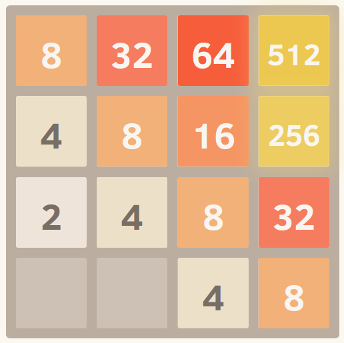
\includegraphics[width=0.15\textwidth]{monotonicity_2048.png}
        %     \caption{Demonstration of a monotonic grid}
        %     \label{fig:monotonicity}
        % \end{figure}

    \end{itemize}

    \begin{algorithm}[t]
        \SetAlgoLined
        initialize\_gamegrid()\;
        \While{game\_over != True}{
            score\_list = new list()\;
            \For{action in actions}{
                score\_for\_action = get\_score\_for\_move(action)\;
                score\_list.append(score\_for\_action)
            }
            index =  get\_max\_score\_index(score\_list)\;
            max\_score\_move = get\_corresponding\_move\_for(index)\;
            gamegrid.play(max\_score\_move);
        }
        \caption{Greedy First Algorithm}
    \end{algorithm} 
    
    \subsubsection{Implementing Heuristics:} 
    In this paper, implementation of three heuristics are done and its behavior is studied in greedy algorithm as well as Monte Carlo Tree Search. The algorithm can be updated with the following expression to accommodate heuristic score while computing next move.

    \begin{multline} \label{heuristic_score_equation}
    Score  = \alpha \times Max \ Score \ of \  Immediate \ Move \\
    + \beta \times Number \ of \ Empty \  Cells \\
    + \gamma \times Weighted \ Matrix \ Multiplication \ Score  + K
    \end{multline}

    In equation \ref{heuristic_score_equation} \(\alpha ,  \beta , \gamma , and K \) are coefficients which helps tune the heuristic function. The combination of these parameters results in weighted heuristic function which can be used to study variation in performance of algorithms.

    \subsection{Monte-Carlo Tree Search (MCTS)}
    
    MCTS is a heuristic search algorithm that is widely used to solve Reinforcement Learning problems. MCTS can find its own moves and explore the environment on its own by randomly playing different moves \cite{mcts_comparison}. The following steps are followed in an iterative fashion to learn the policy of the problem \cite{mcts_medium}.
    
    \begin{algorithm}[t]
        \SetAlgoLined
        Const TREE\_SEARCH\_DEPTH\;
        initialize\_gamegrid()\;
        \While{game\_over != True} {
            score\_list = new list()\;
            \For{action in actions}{
                scores = gamegrid.play(action)\;
                i = TREE\_SEARCH\_DEPTH\;
                \While{i less than 0}{
                      random\_move = get\_random\_move()\;
                    heuristic\_score = get\_heuristic\_score\_for(random\_move)\;
                    scores.append(heuristic\_score)\;
                    i = i - 1 \;
                }
                score\_list.append(average\_of(scores))
            }
            index =  get\_max\_score\_index(score\_list)\;
            max\_score\_move = get\_corresponding\_move\_for(index)\;
            gamegrid.play(max\_score\_move)\;
        }
        \caption{Monte Carlo Tree Search Algorithm}
    \end{algorithm}
    
    \begin{enumerate}

        \item \textbf{{Selection:}} A leaf node from the tree which has the highest probability of maximising the value is selected. The chosen node is usually in the current representation of the tree and this current representation is not always the complete version, as the entire environment may not be explored in one go.
        
        \item \textbf{{Expansion:}} The selected node is expanded and one or more child nodes are added to the tree. These newly added child nodes indicate future moves that can be played later.
        
        \item \textbf{{Play-out:}} A random play is performed starting from a child node that was added during expansion. The play is done until a terminal state is reached or until a fixed depth is reached. Based on the results of the random explorations, each of the child nodes that was expanded is given a reward. The reward is based on the final state reached by the exploration and how close it was to the favoured state.
        
        \item \textbf{{Backpropagation:}} Based on the results obtained at the child nodes, the tree is then traversed back through all the parent nodes while updating their statistics about the moves that could be followed to reach a terminal state. All the parent nodes, including the root node,https://www.overleaf.com/project/5e91ceba1d9c8a000130e528 is updated with the new values. With this new knowledge, the next time an exploitation is required to be done, the most optimal path is chosen based on the current knowledge of the tree.

    \end{enumerate}
    

    % Some of the key properties of MCTS are \cite{mcts_keyProps}:\\

        % \begin{itemize}

        %     \item The search can be performed iteratively for any number of times and yet when it comes to exploitation, a relatively optimal path will be present. Generally, the longer the exploration is performed, the better the final result.

        %     \item An evaluation function is not required as the random nature of the play-out step ensures no moves are ruled out and the relatively optimal path is always known in the tree.

        %     \item The search develops asymmetric trees that prunes sub-optimal paths automatically and can thus look for more optimal paths that could arrive deeper down the tree.

        % \end{itemize}

\subsection{Expectimax Search}
   	
   In this approach, at every agent node (board state) there are 4 chance nodes with expected fitness value representing the future configuration of the board after playing each of the 4 moves: Left, Right, Up, and Down. Expectimax algorithm chooses the move corresponding to the maximum fitness valued chance node. There are three aspects of the heuristic function:

\begin{itemize}
    \item \textbf{Topology:} The mathematical end of the game generates a Snake-Line Pattern \cite{blog_maths_2048}. In an ideal game the two tiles to be combined should be close to one another with no tile in between. Thus, our heuristic function flattens the 2D game board into a 1D sequence of tiles.
    
    \item \textbf{Geometric Series:} All configurations of the tiles are a power of 2. Hence, each tile in the game belongs to the geometric series 2, 4, 8, ..., 2048. Thus, each term in the 1D sequence is weighted by the term in the geometric series and then summed to form the fitness value of the given board state \cite{blog_optimum_2048,blog_maths_2048,gjdanis}. This ensures that the highest valued tile at the desired position should get a high reward.
    
    \item \textbf{Penalty:} In the mathematical end of the game, the highest tile is located at the corner of the board. Thus, we penalize the board state that does not have the highest valued tile at the left corner of the board.
    
    % \begin{figure}[t]

    %     \centering
    %     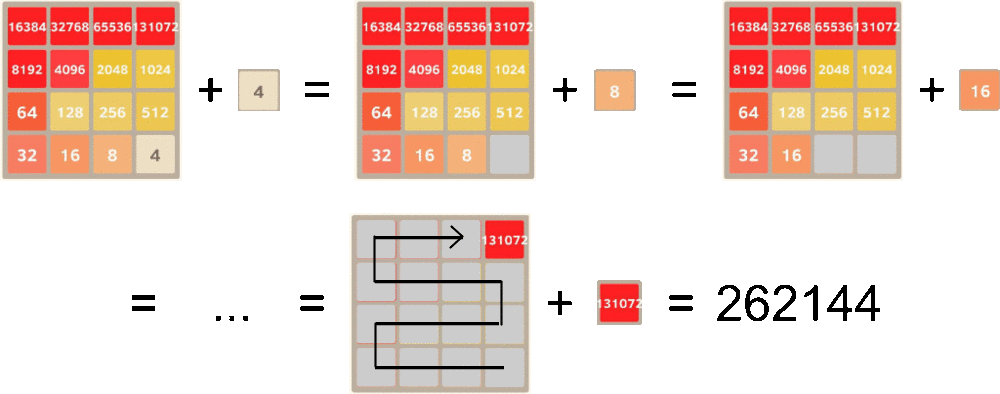
\includegraphics[width=0.25\textwidth]{Sum-of-All-Tiles.png}
    %     \caption{Snake-Line pattern in mathematical end of the 2048}
    %     \label{cMathematical_End_of_2048}
    % \end{figure}
    
\end{itemize}

    \begin{algorithm}[t]
    
        \SetAlgoLined
        % \Function{get\_moves}{board\_state}
        %     \State For each move perform \State \textbf{EXPECTIMAX\_SEARCH(board\_state, depth=4)} and evaluate future configurations of the board recursively for depth 4 \\
        %     \State Store the fitness value for each move in \textit{moves\_fitness\_dictionary} \\
        %     \Return \textit{moves\_fitness\_dictionary}
        % \EndFunction
        
        \Function{evaluation}{board\_state}\\
            Calculate the fitness by implementing Snake-Line Pattern heuristics\; Weigh the flattened sequence with Geometric series\;
            Penalize the board without highest valued tile in lower left corner\;
            \Return \textit{fitness}
        \EndFunction
        
        \Function{Expectimax\_Search}{board\_state, depth, is\_AI\_move = False} \\
            \If{ depth == 0 or no\_move\_exists() }{  
                \Return  \textbf{EVALUATION(board\_state)}
            }
            Calculate fitness using \textbf{EVALUATION(board\_state)}\\
             \eIf{ is\_AI\_move}{
                 Perform recursive\;  \textbf{Expectimax\_Search(child\_board , depth-1)}\\
                 for all moves and calculate its fitness values.\\
            } {
                 For every empty cell in the board spawn two childern (2-tile and 4-tile)\;
                Return weighted (as per 90:10 Distribution) average of the fitness\;  of every  child generated after performing recursive  \textbf{Expectimax\_Search(child\_board\_state , depth-1)}
            }
           \Return \textit{fitness}\;
        \EndFunction \newline
    initialize\_gamegrid()\;
        \While{True}{
            \textit{get\_moves\_fitness\_dictionary(board\_state, depth=n)}\;
            Play the move with maximum fitness\;
            \If{ no\_move\_exists() }{Game Ended}
        }
    \caption{Expectimax Search Algorithm}
    \end{algorithm}
    
    \subsection{Q Learning}
    Q-Learning is a reinforcement learning algorithm which takes actions that are outside of the current policy \cite{watkins1992q}. As such it is considered an 'off-policy' reinforcement learning algorithm. We used Q-learning to experiment with how well reinforcement learning could work with a problem such as 2048. For this we created a Deep Q Network (DQN) based on the works by \cite{dqnGit}. 

    The model is trained using Tensorflow \cite{tensorflow}. It consists of 2 convolution layers, an expansion, and a hidden layer. The first convolution layer consists of 2 convolution 2D tensors, while the second layer uses 4 tensors. The expansion and hidden layer reshapes the output to the required form. 
    			1
    The model was trained with Gamma and Epsilon values of 0.9, and the starting learning rate is set as 0.0005. The replay memory is initialized with 6 GB of memory which is used to sample the minibatch. A RELU activation function was used with an RMSProp optimization function. The Epsilon value is used as a threshold to use greedy approach randomly. After certain intervals, the epsilon value is further reduced. The learning rate also decays exponentially by each episode. The model is trained for 20,000 episodes.
		
    \begin{algorithm}[t]
        \SetAlgoLined
        Initialize hyperparameters and replay memory\;
        Initialize action value function Q with random weights\;	
        \For{episode in 1 to M}{
            Initialize 2048 board
            \While{game is not lost}{
          	    \eIf{epsilon $>$ random value}{
          	    	Set up temporary board \\
        		    Use greedy approach to take action and observe reward \\
        		    Make the action with max reward on the real board \\
          	    }{
          		    Find moves with the max Q value\\
        		    \For{control in Q value table}{
        			    Set up temporary board\\
        			    Take control action and observe reward \\
        		    }
        		    Make the action with max reward on the real board \\
          	    }
          	    Store observations in replay memory \\
          	    \If{replay memory $>$ memory limit}{
              		Back-propagate and sample the mini batch\\
              		Store layer weights
          	    }
          	Reduce epsilon and learning rate values\\
            }
        }
        \caption{DQN Algorithm}
    \end{algorithm}

    \section{Experimental Results}
    % In this project, the game simulations are carried out using TKinter library in python \cite{Tkinter}. The  running game environment setup is referenced from the following source\cite{yangshun}.
  
    \subsection{Methodology}
    Each algorithm is simulated over the same environment. Greedy First, MCTS and Expectimax algorithms are evaluated and compared based on the max score and average score achieved for 100 consecutive runs. The agent is allowed to perform 400 moves in each individual run.  Also, the Game Progression Chart shown in Figure \ref{figure:results}(b) demonstrates how an individual algorithm is able to score as game progresses. For our DQN Agent, we analyze its scores over the number of episodes we trained it for. 
    Instructions for setting up the local environment is given in the repository \cite{AI-RKRS}.
    
    \subsection{Results}
    
    Figure \ref{figure:results}(a) shows that Expectimax algorithm outperformed all the implemented algorithms while Random Moves algorithm sets a baseline for comparison. Greedy Algorithm performed well when compared with MCTS with all heuristics variations. Three variations of heuristic functions mentioned in section \ref{heuristics} are used and its performance in Greedy First algorithm and MCTS algorithm is measured. From game score, it is clear that Empty Cell Heuristics performed better than weighted cell heuristics. 
    
    Figure \ref{figure:results}(b) captures progression of game score in individual runs of implemented algorithms. In Random moves algorithm, the game got over in nearly first 100 moves, whereas gameplay of Expectimax algorithm is still in progression even after performing 400 moves.
    
    Table \ref{depth-analysis} captures the performance analysis of Expectimax alogrithm for different depth limits. It has been observed that the Expectimax search approach achieves a max tile of 2048 at depth 2 by performing 1460 moves. To assess the performance of the Expectimax search we also ran the simulation 10 times at depth 4 and could achieve the 4096 tile more than 60\% of the time. According to figure \ref{figure:results}(a), Expectimax algorithm in its default configuration of depth 1 and 400 limited moves outperforms rest of the AI approaches.
    
    Figure \ref{figure:results}(c) shows the growth in score of DQN agent with the number of episodes. The score is averaged over 100 iterations for better clarity. It should be noted that training for 20,000 episodes took 4 hours of time and achieved a maximum Score of 46976 with 4096 as the maximum tile.

    % \begin{figure}

    %     \centering
    %     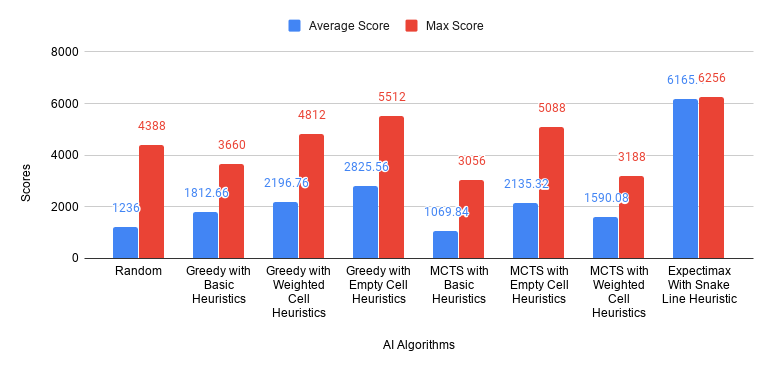
\includegraphics[width=0.5\textwidth]{Comparative Analysis.png}
    %     \caption{Comparative Analysis of Algorithms}
    %     \label{comparative_analysis_of_algorithms}
    % \end{figure}

    % \begin{figure}[h!]

    %     \centering
    %     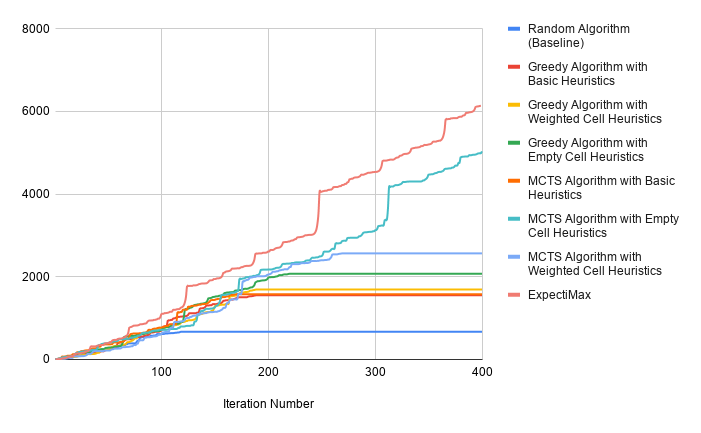
\includegraphics[width=0.5\textwidth]{Game Score Progression Chart.png}
    %     \caption{Game Score Progression Chart}
    %     \label{game_score_progression_chart}
    % \end{figure}
    
    % \begin{figure}[h!]

    %     \centering
    %     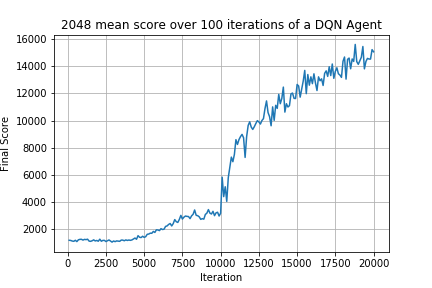
\includegraphics[width=0.5\textwidth]{dqn-mean-iteration-score.png}
    %     \caption{DQN Mean Iteration Score}
    %     \label{dqn meaen iteration score}
    % \end{figure}
    \begin{table}[t]
    \centering
    \caption{Expectimax Search: Depth Analysis}
    \label{depth-analysis}
    \begin{tabular}{|c|c|c|c|c|}
        \hline
        Depth & Max-Tile & Moves & score & Execution Time (min)\\
         \hline 
    1 & 256  & 238  & 2804   & 0.03   \\
    2 & 2048 & 1460 & 27844  & 0.29   \\
    3 & 2048 & 1862 & 35932  & 1.25   \\
    4 & 8192 & 5594 & 132780 & 31.65 \\
     \hline 
        \end{tabular}
        \end{table}
        
    \begin{figure}[h!]
    \centering
    \subfloat[Comparative Analysis of Algorithms]{{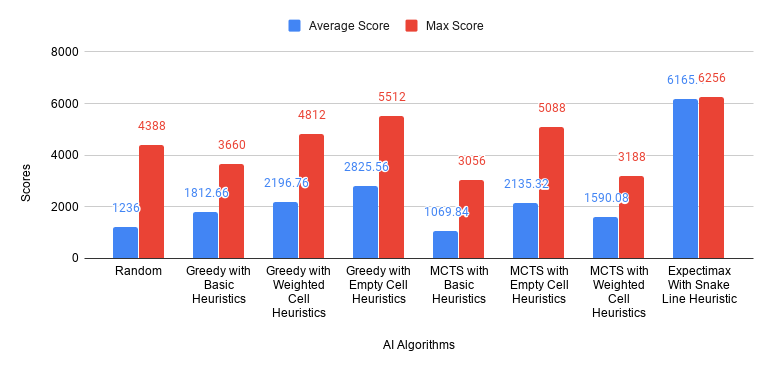
\includegraphics[width=10cm]{Comparative Analysis.png} }}%
    \qquad
    \subfloat[Game Score Progression Chart]{{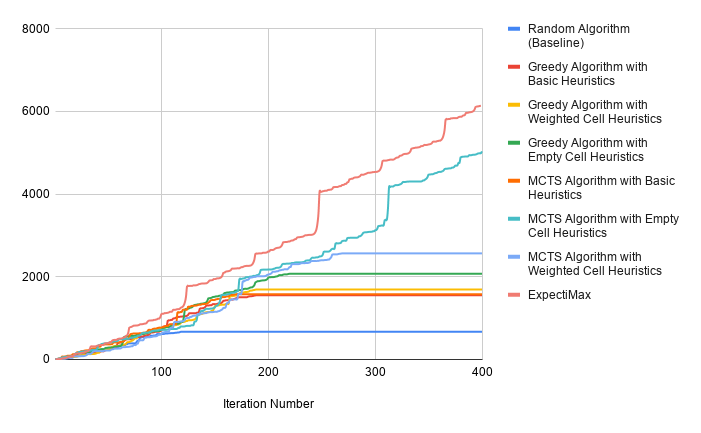
\includegraphics[width=5cm]{Game Score Progression Chart.png} }}%
    \qquad
    \subfloat[DQN Mean Iteration Score]{{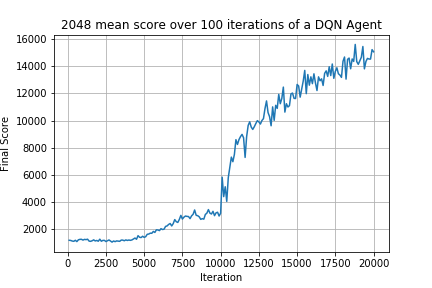
\includegraphics[width=5cm]{dqn-mean-iteration-score.png} }}%
    \caption{Results}%
    \label{figure:results}%
    \end{figure}

    \subsection{Discussion}
    % The greedy first approach is definitely better than a random move approach but its not always the case.
    % Consider the following situation,
    % \begin{figure}[h!]

    %     \centering
    %     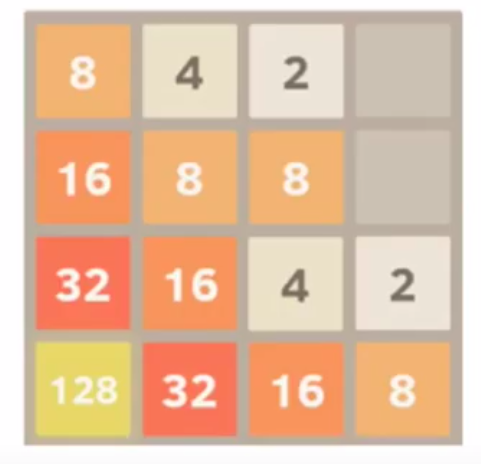
\includegraphics[width=0.15\textwidth]{greedy_img_correction.png}
    %     \caption{Demonstration of a game state when Greedy approach fails}
    % \end{figure}
    

    % The greedy first approach will take \textbf{LEFT} action in order to increase the final game score. In such cases, swiping \textbf{UP} then swiping \textbf{LEFT} is a better than swiping \textbf{LEFT} in the first place. In order to improve the greedy first algorithm, we introduce heuristics which helps agent take appropriate action based on the strategies and rewards assigned for the chosen strategy.
    From the visualizations it seems clear that Expectimax algorithm performs best, given it has both the highest max as well as average score of all the algorithm configurations. Greedy algorithm also outperforms MCTS. This could be because the Play-out happens randomly in MCTS algorithm. The level of randomness is more in MCTS when compared with Greedy approach. Our DQN agent does manage a decent maximum score, but it takes a longer training period and even then does not beat out Expectimax in terms of maximum achieved score and max tile.
    
    Depth limited Expectimax Search approach solved the 2048 problem in polynomial time. Since we take a weighted average of all children nodes obtained in the depth limited recursive search, we did not apply alpha-beta pruning \cite{7162574} to get rid of the branches thus reducing the search space. This could have further improved our score. The weight matrix mentioned in equation \ref{weighted_score_equation} may not be the most ideal, it only helps illustrate the choice of the underlying heuristic. It is possible to use other optimization methods, such as Genetic Algorithms and Particle Swarm Optimization (PSO), which is currently out of scope of this paper.
    

    \section{Conclusions}
    2048 is an extremely uncertain game as the randomly generated new tile after each move is unpredictable. From the experiments it is noted that improving the speed of the algorithm will allow the agent to reach a greater depth in the search tree thereby giving better accuracy. Also, storing the entire game-grid in the form of a bitvector will help save memory and can improve the performance of the agent. In this paper, only a single heuristic is considered at a time by tweaking the values of alpha, beta and gamma from the equation. Future work in this domain could include a combination of several heuristics using weighted coefficients, the use of monotonicity, increasing the smoothness of game-grid and experimenting with heuristics could reveal other ways in which the game play could be improved. Deep learning methods may perform better for larger inputs such as Atari games. Also, a pre-trained model would probably perform better.
    
    In conclusion, the results of the experiments show that Expectimax proves to be the best algorithm out of the chosen ones to win a game of 2048. It is also observed that in general, the greedy approach performs better than the random moves approach. Due to this, it is believed that the MCTS algorithm is not as efficient as the others. Deep Q-Network is also does not seem to be the most suitable model for 2048 given its low score for its 4 hour training time. 

    \bibliography{ai_doc}
    \bibliographystyle{ieeetr}

\end{document}
